\documentclass[a4paper,hidelinks]{article}
\usepackage{bnaic}
\usepackage[T1]{fontenc}
\usepackage[utf8]{inputenc}
\usepackage{natbib}

\usepackage{filecontents}
\usepackage{hyperref}
\usepackage{graphicx}


\title{\textbf{\huge Traffic Memory: A Multi Agent System Approach to Traffic Flow Optimization}%
}
\author{
	Wouter Reckman (s2231166) \and
    Matthia Sabatelli (s2847485) \and
    Gereon Vienken (s2738805) 
}
\date{}

\pagestyle{empty}

\begin{document}
\ttl
\thispagestyle{empty}

%\bibliography{dmas-gereon_matthia_wouter-traffic_memory-report}


\begin{abstract}
\noindent
In this paper we present a Multi-Agent System simulation of traffic in which 147 agents travel for 10 days in a 7x7 grid, moving from a randomized starting position to a randomly assigned destination. The grid symbolizes a Manhattan-like city consisting of junctions. The number of agents able to move through these junctions during each (discrete) time step is limited, thus creating bottlenecks which in turn may cause traffic jams. This regards the first part of the experiment, in the second part we provide the agents with a memory system enabling them to remember the most congested junctions. Using a weighted A* path finding algorithm they can avoid these and potentially the amount of traffic jams occurring could be reduced. Our results however, showed the opposite effect, which we attribute to a form of cut-through driving arising.
\end{abstract}


\section{Introduction}
During the past decades, travel by car has always been one of the most comfortable and appreciated ways to move through countries and the amount of traffic is ever increasing. Several reasons of this constant growth can be indicated, ranging from the constant increase of affordability of cars, enabling almost every family to own one or several cars, to the creation of the European Community which has led to the elimination of boundaries between countries and has facilitated the trade and exchange of resources between different nations.

As a result, millions of people suffer everyday from congestion and traffic jams in urban road networks while travelling to their daily destinations. Possibly, this happens due to existing road networks and the traffic light systems being outdated and not up to the task of regulating the vastly increased quantity of car traffic of the 21st century. Another possible cause is the tendency of drivers occupying these road networks to exhibit selfish behaviour instead of cooperating to make traffic flow more liveable.

It is desirable to minimize the amount of traffic congestions, because it has several negative impacts. Firstly, it leads to frustration and selfish or even aggressive behaviour of traffic participants in an attempt to move through the traffic faster. \\
Secondly, exhaust gases have a severe negative ecological impact on the environment. Air pollution has in fact reached such high levels that in some countries it has been identified as one of the main reasons of the exacerbation of asthma, allergy and many other respiratory diseases. As described in \cite{ghose2005assessment}, part of the air pollution is caused by the automobile exhausts that, combined with certain industrial pollutants, produce photochemical reactions which in turn damage human health. \\
Even though most people do not think about all these issues, traffic has a very important role in society and this has led to the work that is presented in the next sections.


\subsection{Problem}
The main problem addressed regards the inefficiencies in traffic. Much research has been done in this field by various scientists and as will be explained in more detail in the next section, the flow of traffic has been modelled under various conditions in order to measure its relative impact. This paper attempts to add to this reservoir by trying to understand what possible impact driver memory of previous travels in repeating traffic situations may have. Many of us know the situation of facing traffic jams on their daily commute. What this experiment investigates is what impact recurring jams at the same intersections day after day have: will they still decide to drive the same route and and thus also add to the already existing congestion? Or would they attempt to alleviate it by deciding to find a different route the next time? This article tries to get closer to an answer for this question.

\subsection{State of the art}
In literature, a large amount of research that deals with the optimization of traffic flow may be found and it is mainly possible to divide the approaches that guide this type of research into two sub-fields which both naturally suit the artificial intelligence agent paradigm. On the one side there is research that focuses on modelling the single agents moving through the streets (microscopic models): the main idea of this approach is that by modifying their behaviours, the overall situation of traffic will change as a consequence. This approach may be defined as reductionistic since it deals with the single agents on the streets in order to get an overall improvement of the whole traffic flow. \\
On the other side there is research that tries to model the overall behaviour on the streets without directly influencing the single agents (macroscopic models); this is done by putting focus on external agents that govern traffic, most commonly traffic lights. \\
This last category is the most intuitive and easy to understand, since in everyday life we continuously deal with traffic lights. In fact one does not need to be an expert to understand how a traffic light system works. Most often it is based on a traffic signal timing plan where various traffic phases are coordinated by the system; this is done in order to prevent crashes between traffic phases and ensures the smoothness of the overall traffic flow within the traffic network. As explained in \cite{chin2011q}, there are various ways in which these systems work but the most general approach is that there is a fixed-time traffic signal plan management where all the duration of the traffic signals are pre-set in the database and being executed repeatedly. The configurations of the traffic signals durations are based on historical traffic statistics, gathered over a long period of time. The setting of the fixed time traffic signal plan is not changed until the next review on the traffic statistics is provided.

This is a very common approach, but as highlighted in the paper a, it is too static in some situations. In order to improve the way in which the traffic light system works, the authors have provided the system with a reinforcement learning algorithm, enabling it to adapt itself to the traffic flow it deals with. This is of course a possible way to model traffic flow. The new experiment in this paper though, has been inspired by the microscopic approach explained first.

The main article that guided this work was proposed by Gabel et al. in 2008 \cite{gabel2012cooperative}. In this paper, the authors compared two microscopic traffic simulations that regarded two types of possible drivers: one selfish driver model and one selfless driver model. They showed that the selfish drivers simply tried to maximize their own speed without paying attention to other drivers or the general road situation. Doing so, the probability that traffic jams occurred was very high since there was no cooperation between the various agents on the streets. On the other hand, selfless drivers were also simulated, using a Markov decision model in order to maximize the general velocity over all cars. Doing so, it is true that every agent tried to minimize its personal costs but at the same time bears in mind that there are other agents as well on the streets and is able to find a compromise in order to do not get stuck in traffic. We were very inspired by this approach that tries to verify the impact of other persons in traffic simulations. \\
As will be explained more in detail in the next sections of this paper we decided to provide our agents with a memory system that allowed them to remember situations in which they had to deal with traffic jams. Bearing these in mind they are able to come up with different driving strategies that may be less fast, but optimize the general traffic flow.

This kind of compromise may be seen in different research papers as mentioned by France et al. \cite{france2003multiagent}: coordination between the different agents on the streets is of key importance since it is crucial to maintain a balance between optimized events both at a global level then at a local one. Unfortunately this kind of approach is also very difficult to implement since optimizing local events does not necessarily guarantee a global balance.         

\subsection{New idea}
The new idea of our project proposal is to see if memory can actually have an impact on the flow of traffic over longer periods of time. Thinking about this project we came up with the idea that this may also deal with theory of mind but this link is not directly mentioned in this work, however it may provide an interesting approach for further research. This paper has been guided by the hope that our implementation can show that with providing the agents with some memory in order to avoid previously encountered situations, the traffic flow over the map will go smoother and that the average travelling speed per car will increase. Moreover it is important to highlight that in contrast to our main reference paper \cite{gabel2012cooperative} we only use selfish agents, but by making them more intelligent to pursue their own goals we hope that as an indirect result they will help other agents in the overall process as well.

\section{Method}
\subsection{Simulation model}
The model as used in the base article is a commonly used car following model called the Krauss model, published in \cite{krauss1998microscopic}. This uses a limited number of parameters controlling the distance agents want to keep to their predecessor, their desired velocity, and maximum acceleration and breaking capacities. They run their simulation on a circular road, without intersections and with only a single lane. \\
Since the follow-up experiment described in this article requires agents to have choice in planning their route, a grid road pattern was chosen. Although extensions to the Krauss model have been developed to support this, it was too complex to implement this given the limited time-scope of this project. Instead, a simpler model has been implemented, which is described in the remainder of this subsection.

The model consists of a 7 by 7 grid of intersections. Each of those has a maximum capacity of agents it can hold simultaneously, set to 3. The maximum number of agents in the system is thus $7*7*3=147$ agents. This value is also the amount of agents which can travel through the junction per time step. Leading away from each junction to its neighbouring junction is a street, which has a maximum throughput capacity, set to 5. \\
Time is modelled as days, which consist of 30 time steps, giving enough time for agents to travel the longest possible route (i.e., a Manhattan distance of $7*7$ junctions). \\
The agents restart their route every day, computing their route using the A* algorithm. Their routes are randomly generated at the start of each simulation run. Depending on whether memory has been enabled, this is either non-weighted or weighted using jam counters for each junction.
Figure \ref{fig:grid} shows a visualization of the grid, green indicating empty cells and red indicating cells having reached their capacity.

\begin{figure}[ht!]
\centering
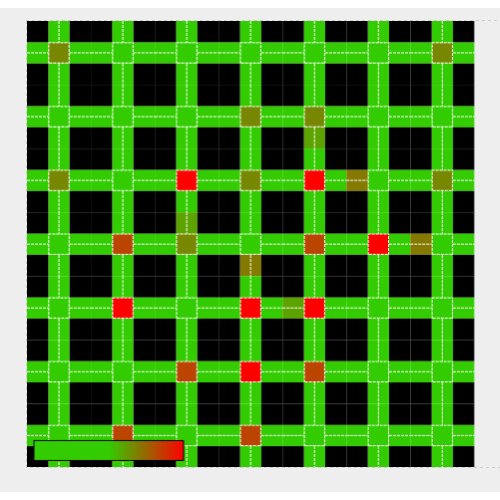
\includegraphics[width = 0.7\linewidth]{grid}
\caption{Traffic Scenario \label{fig:grid}}
\end{figure} 

Traffic jams can occur if agents try to enter a junction from multiple directions and then try to leave it simultaneously, this way the junction can become a bottleneck. This aspect of the model is makes the comparison possible. When memory has been enabled, at the end of the each simulation day the agents remember the how many jams occurred in each junction and for the following day they use this information to re-plan their routes avoiding the most busy locations. \\
The memory has been implemented as a global model, so agents all use the same information, as if this has been shared for instance by Internet-enabled navigation systems.

\subsection{Experiment design}

The output produced by the experiment is the total number of jams occurring in each part of the simulation. First the base simulation using a regular A* path finder, then the second part which uses weighted A* to implement memory.
During the simulation this amount of jams that have occurred is saved for every time step over a period of 10 days. This process is repeated a 100 times in order to avoid effects due to chance, as the agent routes are randomized at the start of each simulation. \\
In the next section the graphs that represent this simulation are discussed in order to show how the amount of jams has decreased over time when the agents were provided with memory.  

%---TODO: beschrijving van tabel hier laten? maar zeggen dat we alleen het aantal files gemeten hebben (stuck TS is daar een andere weergave van)
%During the 10 days of the 2 simulations we have measured and tracked the following parameters for every agent. First of all the starting point and the destination point that have been randomly assigned in order to get an idea where the agents needed to go. We also have measured the relocation process in order to see if and how they are moving, but the most important data comes from the Stuck TS parameter that measures how much each agent that is blocked in traffic is waiting before being able to reach its destination. We also have kept track of the overall distance that each agent has covered during its travelling period, the highest this parameter is, the more likely it is that the agent has bumped into a traffic jam. These parameters are all shown in figure \ref{fig:measurements}.
%
%\begin{figure}[ht!]
%\centering
%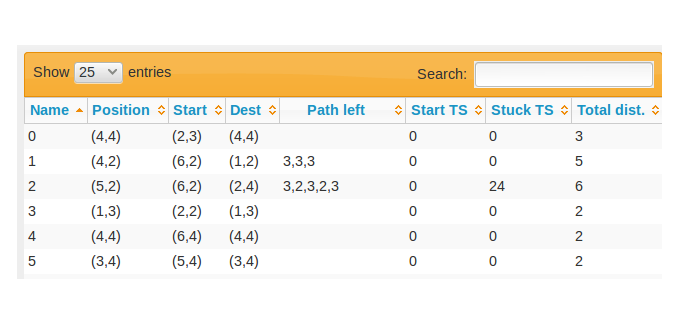
\includegraphics[width = 1.0\linewidth]{data}
%\caption{Measurements Table \label{fig:measurements}}
%\end{figure} 


\section{Results}
\subsection{Experiment findings}
Contrary to the hypothesis, the experiment shows that the addition of memory has an adverse effect on traffic flow. Figure \ref{fig:jam-progression} shows that without memory, jams occur at the beginning of each day but these subside as agents reach their destination. With memory however, the amount of traffic jams occurring is ever increasing, possibly even causing agents not to reach their destination on the same day. \\
One remark considering the graph: it may be slightly misleading since the data shown is cumulative. In other words, the lines show the total amount of jams occurred over the whole simulation time, so the simulation with memory enabled might look worse than it actually is.

\begin{figure}[ht!]
\centering
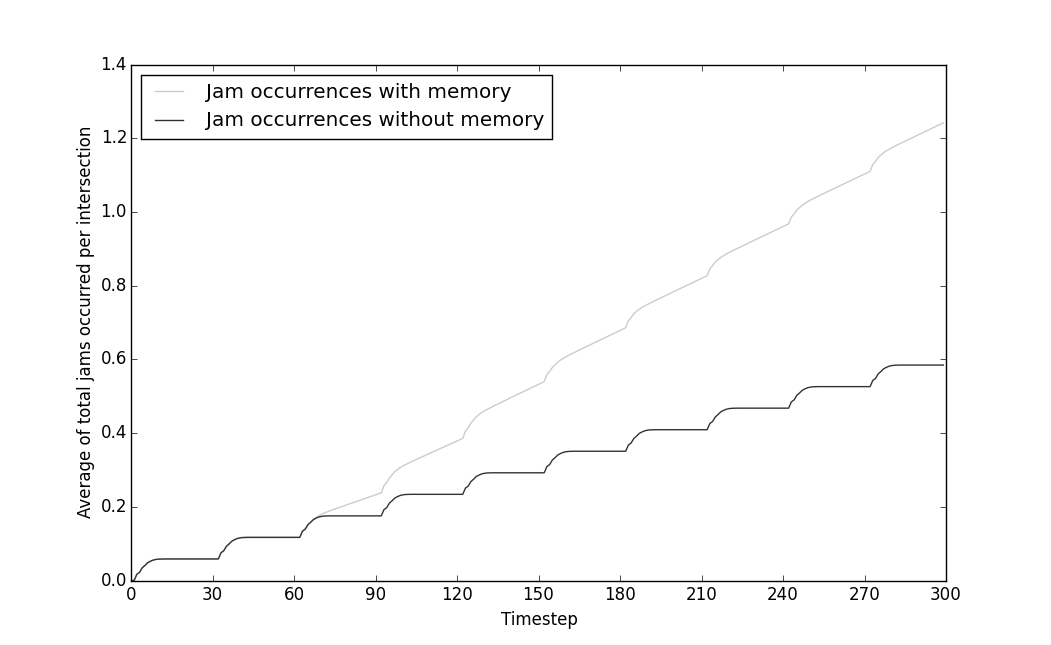
\includegraphics[width = 0.7\linewidth]{100sims-mem-vs-nomem}
\caption{Progression of traffic jams over time \label{fig:jam-progression}}
\end{figure} 

\subsection{Interpretation of findings}
As noted, the outcome of the experiment is opposite to the hypothesis that the addition of memory would decrease the amount of traffic jams. One explanation for this behaviour is that since agents all try to avoid the same bottlenecks, they also tend to take the same detours, resulting in what is commonly known as cut-through driving. As all agents do this, the bottlenecks do not disappear, but shift to different locations.

\section{Conclusion}
The conclusion that can be drawn from this experiment is quite simple: only adding memory to route planning of traffic participants does not help reduce the amount of traffic jams. In fact it seems to make the situation worse.

\subsection{Discussion}
Although further investigation would be required to establish that cut-through driving is actually causing the increased occurrence of traffic jams, it might very well be a plausible explanation. Not without reason do inhabitants of areas around busy roads, or roads with long-term construction work often complain about this behaviour of passing drivers and do local governments take measures to counteract this.

A possible next step to this experiment would be to add theory of mind. If agents reason about the jam-avoiding behaviour of others, they might come up with solutions to all take the same detour. For instance, they could add a little randomization to their route to that in total the traffic load will be spread more evenly.

\subsection{Relevance}
The intention of this experiment is to determine if the use of memory in a repeated traffic situation can improve flow and prevent jams. This information could be used to improve traffic guidance systems like GPS navigation. If applying local memory (in the sense that there is no cooperation) to agents can improve traffic flow, that would mean that even such a selfish change could cause improvement to the global situation. \\
If that is not the case however, it would be required for agents (or navigation systems) to have communication between each other in order for the traffic system as a whole to improve. Such distribution of information would be far more difficult to implement with current technology.

The benefit of an easy solution could be that improved guiding systems can be produced which allow optimization of traffic for everyone. The benefits of such optimized traffic are widely known, as mentioned in \cite{france2003multiagent}. Not only is the negative influence on personal health of traffic-induced stress an important factor, but it also hurts the economy when people spend more time in traffic than necessary, being unproductive at that time. On a global scale, optimizing traffic and the related reduction of carbon emission is beneficial to the environment. \\
All in all, optimising traffic is a worthwhile attempt to promote peoples health productivity and quality of life. 

%\section{Acknowledgements}

\bibliographystyle{plain}
\bibliography{dmas-gereon_matthia_wouter-traffic_memory-report.bib}


\end{document}
